\section{Sistemi di Processi}
È spesso conveniente scomporre un processo in $n$ sottoprocessi dando vita ad un sistema di processi, questo può permetterci di parallelizzare le operazioni pur rispettando l'ordine di esecuzione.

\begin{note}
    Possiamo utilizzare un grafo per rappresentare le relazioni di precedenza tra i processi, i nodi del grafo sono i sottoprocessi e un arco rappresenta una relazione di precedenza.
\end{note}

\subsubsection*{Esempio 4.1.}
Vogliamo risolvere l'equazione $f = (a + b) \cdot (c + d) + e$, possiamo risolverlo:
\begin{figure}[H]
    \centering
    \begin{minipage}{0.45\textwidth}
        \centering
        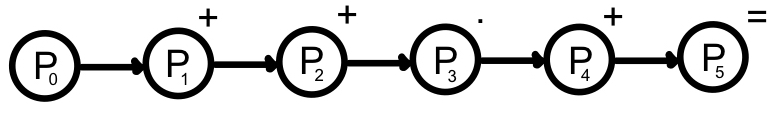
\includegraphics[width=\linewidth]{assets/math-sequenziale.jpeg}
        \caption{In modo sequenziale}
    \end{minipage}
    \hfill
    \begin{minipage}{0.35\textwidth}
        \centering
        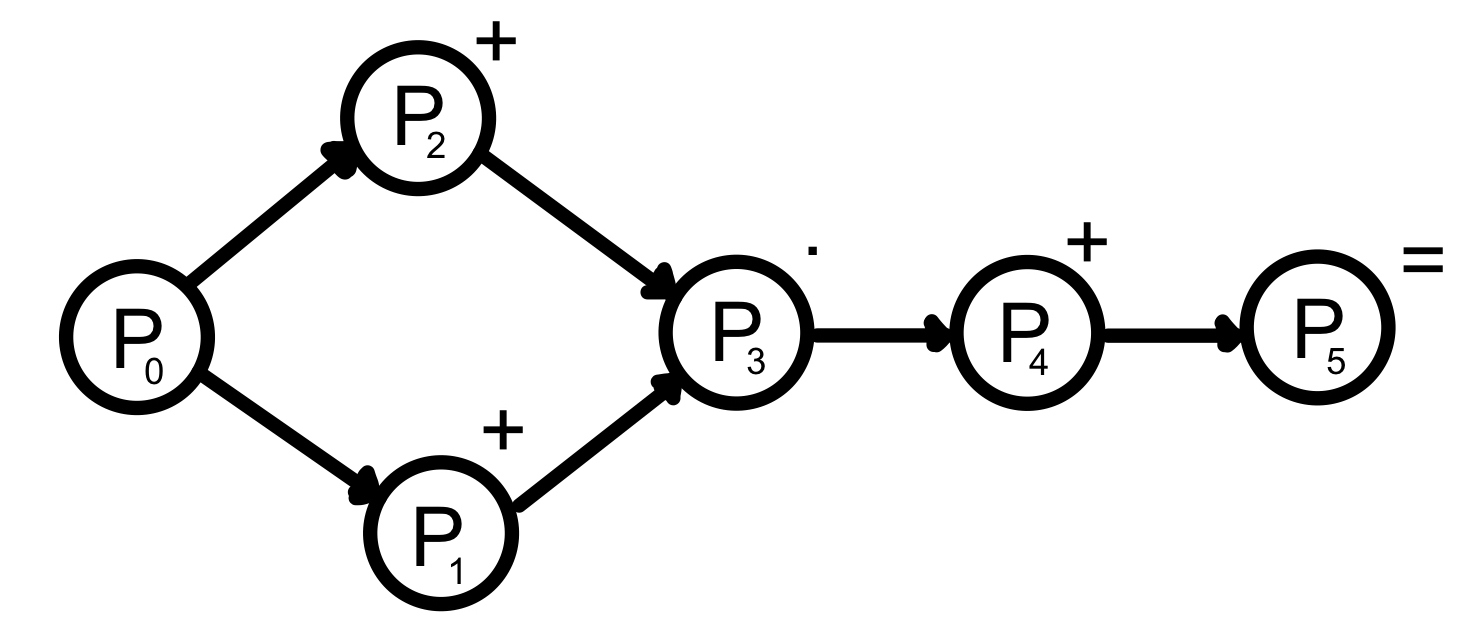
\includegraphics[width=\linewidth]{assets/math-parallelo.jpeg}
        \caption{In parallelo}
    \end{minipage}
\end{figure}

\subsubsection*{Esempio 4.2.}
Conoscendo i tempi di esecuzione di ogni singolo processo possiamo anche calcolare la quantità di tempo che viene risparmiata parallelizzando l'operazione.

\begin{figure}[H]
    \centering
    \begin{minipage}{0.45\textwidth}
        \centering
        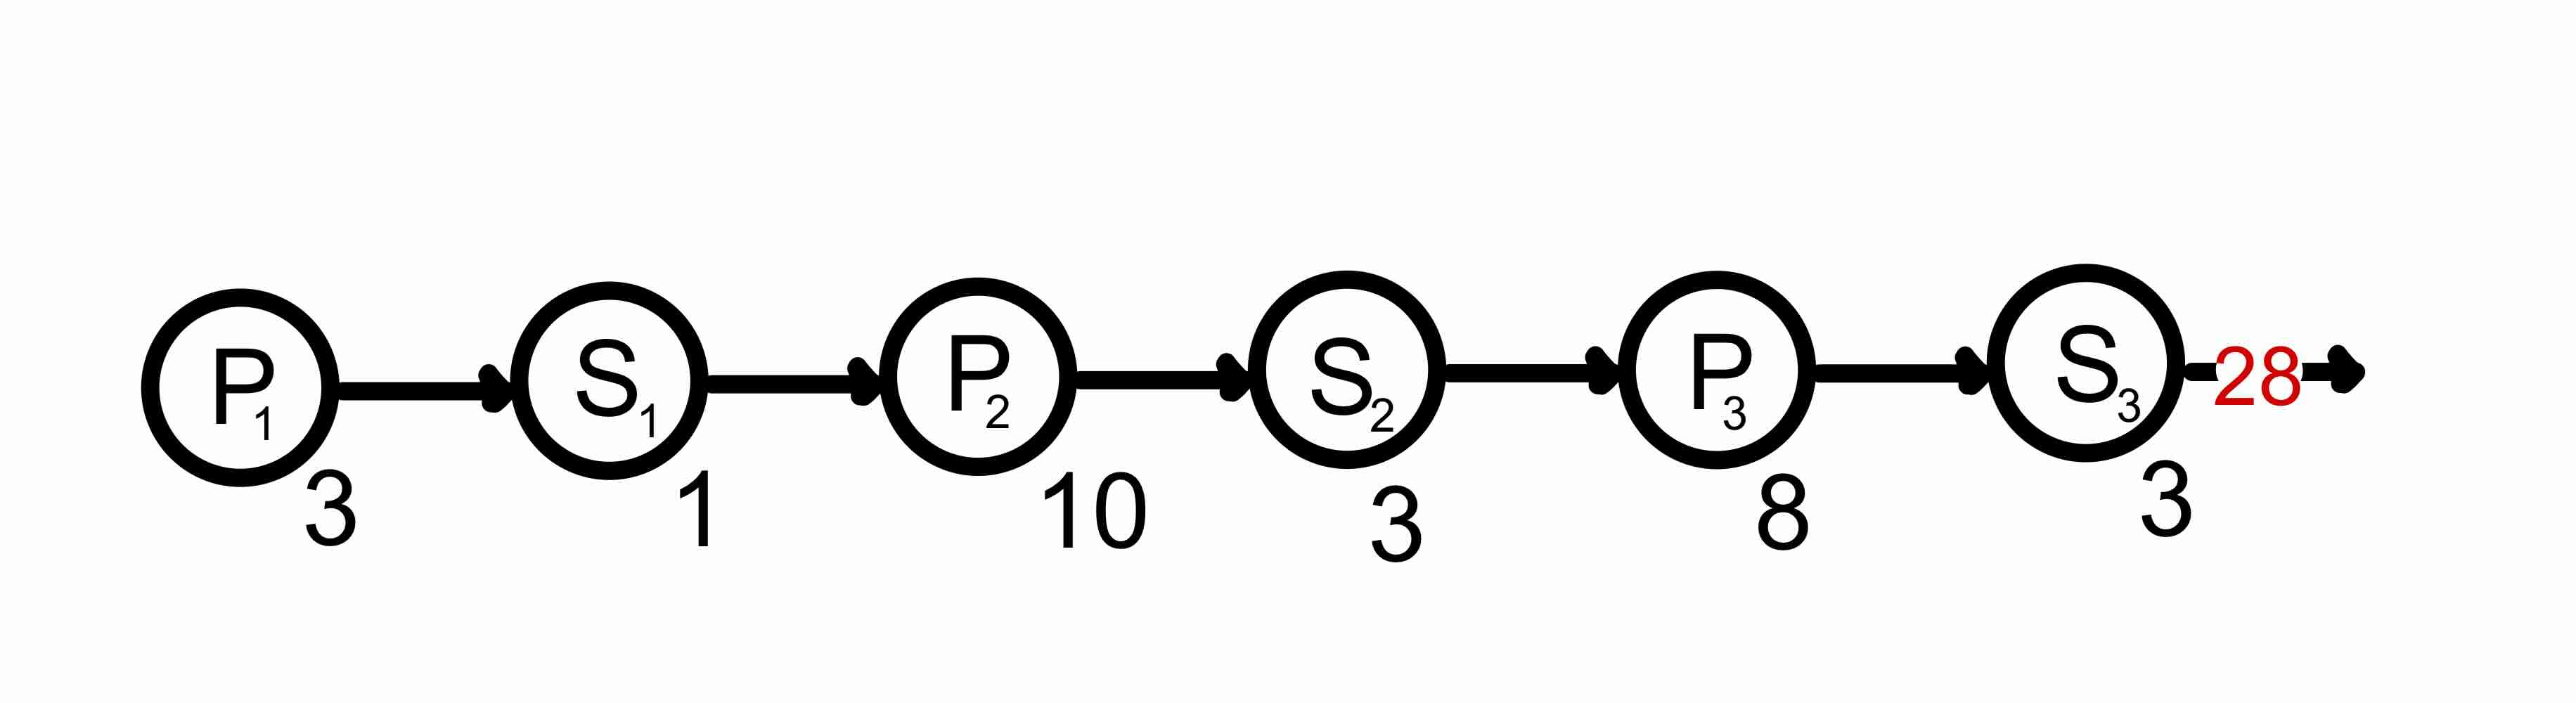
\includegraphics[width=\linewidth]{assets/threads-sequenziale.jpeg}
    \end{minipage}
    \hfill
    \begin{minipage}{0.35\textwidth}
        \centering
        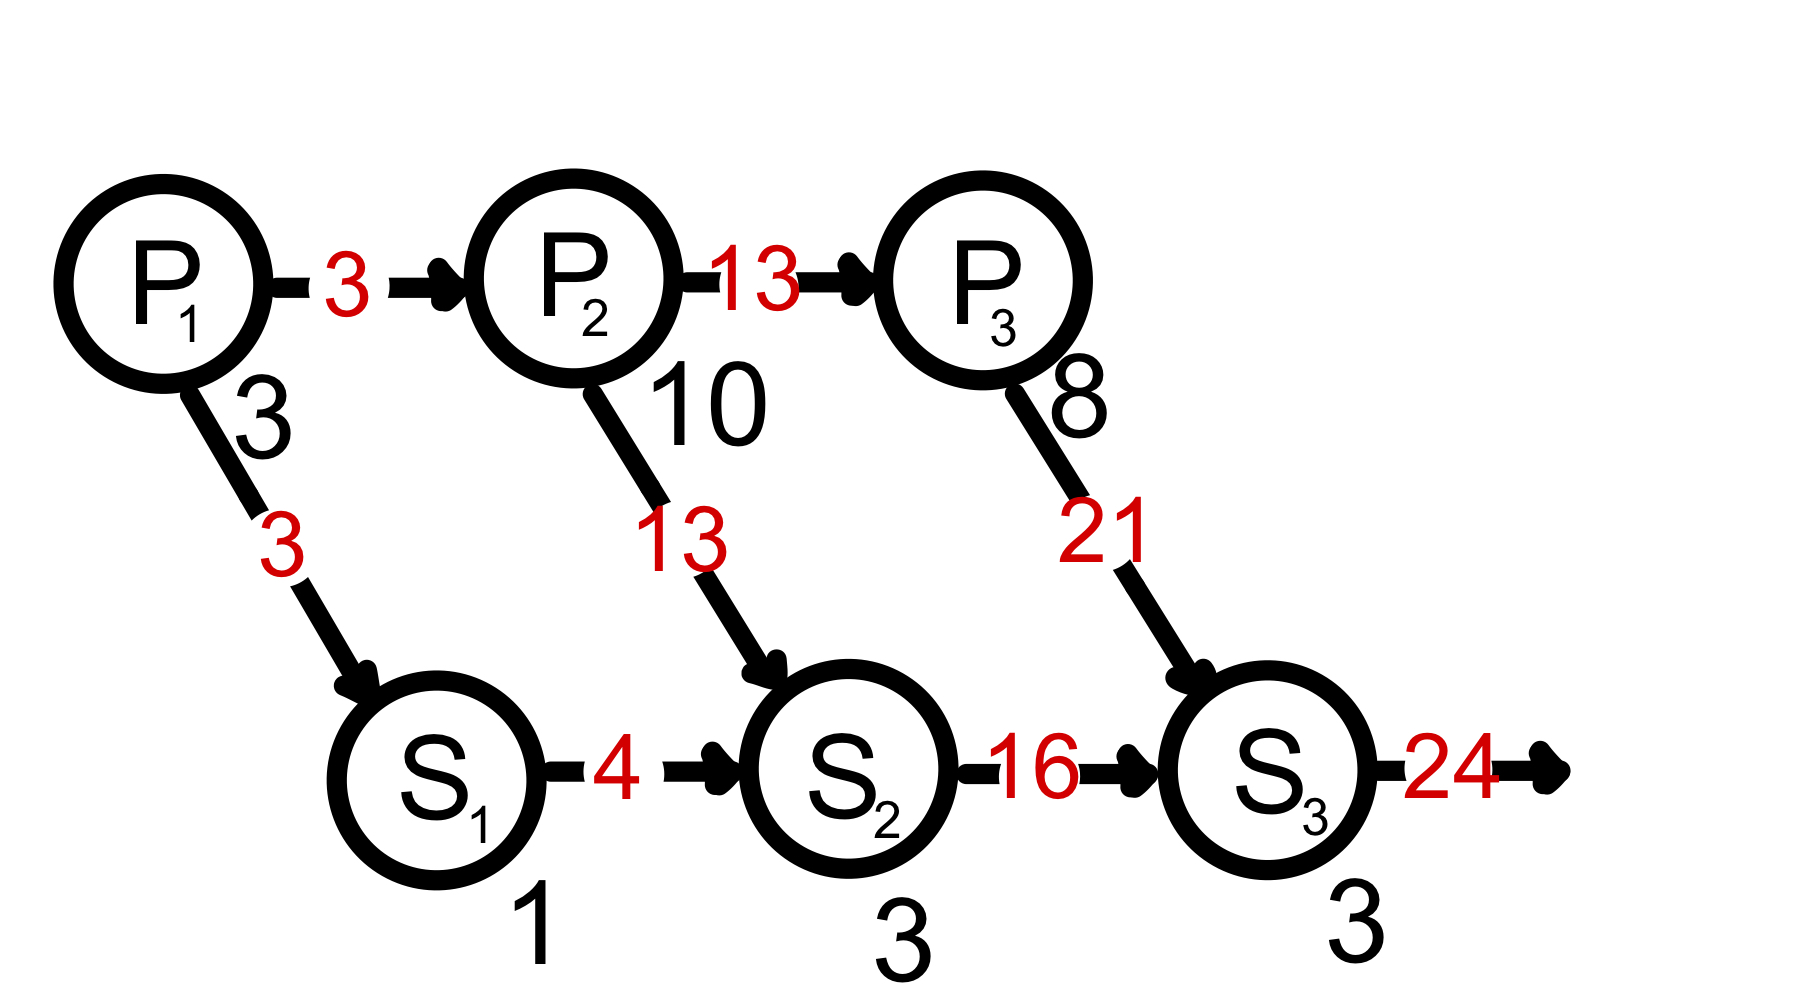
\includegraphics[width=\linewidth]{assets/threads-parallelo.jpeg}
    \end{minipage}
    \caption{Aumento di efficienza ottenuto parallelizzando il processo}
\end{figure}

\subsection{Sistemi Chiusi e Aperti}

Un sistema si definisce \textbf{chiuso} se esiste un singolo processo iniziale e un singolo processo finale.

Il sistema è \textbf{aperto} se non è chiuso.

\spacer

Due sistemi di processi possono essere combinati in \textbf{serie} o in \textbf{parallelo}.

\begin{figure}[H]
    \centering
    \begin{minipage}{0.45\textwidth}
        \centering
        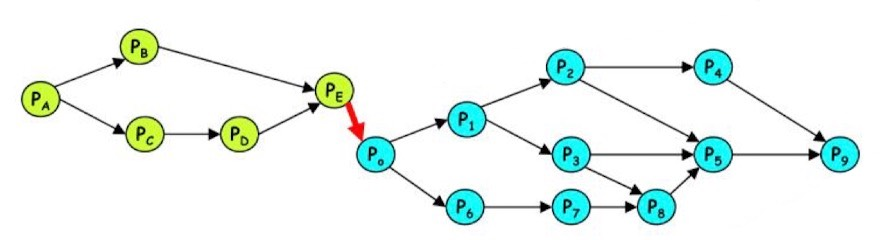
\includegraphics[width=\linewidth]{assets/sistema-serie.jpg}
    \end{minipage}
    \hfill
    \begin{minipage}{0.45\textwidth}
        \centering
        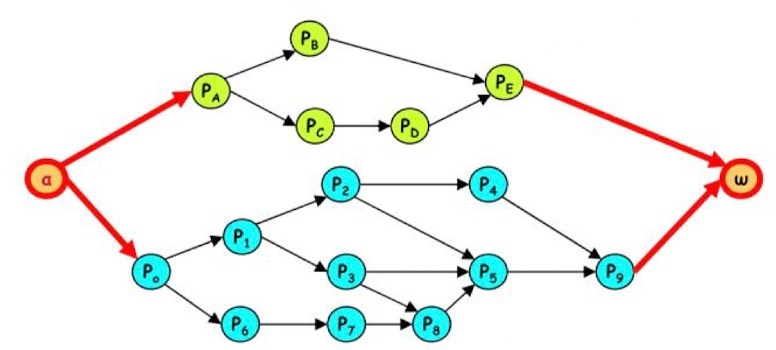
\includegraphics[width=\linewidth]{assets/sistema-parallelo.jpg}
    \end{minipage}
\end{figure}

\begin{note}
    I grafi ci permettono di trovare anche il \textbf{massimo grado di parallelismo} che un sistema raggiunge, si può trovare osservando il numero di processi nella stessa colonna.

    Nel caso rappresentato qui sopra ci sono al massimo 3 processi ponendo i sistemi in serie e 5 processi ponendo i sistemi in parallelo.
\end{note}

\subsection{Determinatezza}

Un sistema si dice \textbf{determinato} se le diverse velocità dei processi e l'ordine di esecuzione dei processi non influenzano il risultato.
Altrimenti si dice che il sistema è \textbf{indeterminato}.

\subsection{Inferenza}
\begin{note}
    Possiamo associare ad ogni processo un \textbf{dominio} contenente i dati su cui esso lavora e un \textbf{codominio} che contiene i risultati del processo.

    La \textbf{funzione mappa} trasforma elementi del dominio in elementi del codominio.
\end{note}

Due processi si dicono \textbf{non inferenti} se almeno una delle due osservazioni è corretta:
\begin{sitemize}
    \item Uno è il successore all'altro
    \item Non si intersecano i condomini e neppure i domini con i condomini.
\end{sitemize}

\subsubsection*{Proprietà}
\begin{sitemize}
    \item Condizione necessaria e sufficiente affinché un sistema sia \textbf{determinato} è che sia composto da processi \textbf{non inferenti}.
    \item Due sistemi sono \textbf{equivalenti} se sono costituiti dallo \textit{stesso insieme di processi}, sono \textit{determinati} e partendo dallo \textit{stesso input} producono lo \textit{stesso output}.
\end{sitemize}
